\documentclass[aspectratio=169]{beamer}
%\documentclass[aspectratio=43]{beamer}

\usepackage{graphicx}  % Required for including images
\usepackage{natbib}
\usepackage{booktabs} % Top and bottom rules for tables
\usepackage{amssymb,amsthm,amsmath}
\usepackage{exscale}
\usepackage{natbib}
\usepackage{tikz}
\usepackage{listings}
\usepackage{color}
\usepackage{bm}
% Setup TikZ
\usepackage{tikz}
\usetikzlibrary{arrows}
\tikzstyle{block}=[draw opacity=0.7,line width=1.4cm]
% Setup hyperref
\usepackage{hyperref}
\hypersetup{colorlinks=true}
\hypersetup{citecolor=porange}
\hypersetup{urlcolor=porange!80!}
\hypersetup{linkcolor=porange}

\newtheorem{proposition}{Proposition}
\newtheorem{remark}{Remark}
\newtheorem{principle}{Principle}

%% Writing quarters
\newcommand{\wQ}[1]{{\textcolor{white}{Q#1}}}
\newcommand{\bQ}[1]{{Q#1}}

% Uncomment appropriate command to disable/enable hiding
\newcommand{\mypause}{\pause}
% \newcommand{\mypause}{}
\newcommand{\myb}[1]{{\color{blue} {#1}}}

\DeclareMathAlphabet{\mathpzc}{OT1}{pzc}{m}{it}

%% Autoscaled figures
\newcommand{\incfig}{\centering\includegraphics}
\setkeys{Gin}{width=0.9\linewidth,keepaspectratio}

%Make the items smaller
\newcommand{\cramplist}{
	\setlength{\itemsep}{0in}
	\setlength{\partopsep}{0in}
	\setlength{\topsep}{0in}}
\newcommand{\cramp}{\setlength{\parskip}{.5\parskip}}
\newcommand{\zapspace}{\topsep=0pt\partopsep=0pt\itemsep=0pt\parskip=0pt}

\newcommand{\backupbegin}{
   \newcounter{finalframe}
   \setcounter{finalframe}{\value{framenumber}}
}
\newcommand{\backupend}{
   \setcounter{framenumber}{\value{finalframe}}
}

\usetheme[bullet=circle,% Use circles instead of squares for bullets.
          titleline=true,% Show a line below the frame title.
          ]{Princeton}

\title[{\tt }] {Lecture 13: Software and Hardware Issues in Computational Physics}%
\author[https://apc523-2020.rtfd.io]%
{Ammar H. Hakim ({\tt ahakim@pppl.gov}) \inst{1}}%

\institute[PPPL]
{ \inst{1} Princeton Plasma Physics Laboratory, Princeton, NJ %
}

\date[3/23/2020]{Princeton University, Course APC523, 2020}

\begin{document}

\begin{frame}[plain]
  \titlepage
\end{frame}

%----------------------------------------------------------------
\begin{frame}{Goal: Hardware and software for Computational Physics}
  Our computation physics codes must run somewhere: Making code work
  on modern hardware and writing \emph{long-lived} and \emph{usable}
  software is highly non-trivial task. {\bf Difficult
    and under appreciated art!}
  \mypause%
  \begin{itemize}
  \item Modern computer hardware is changing: new architectures are
    emerging (too) rapidly.
    \begin{itemize}\cramplist
    \item Pressure on hardware: make chips \emph{faster} but
      \emph{consume less energy}. Contradictory goals.
    \item New directions: many (100s or 1000s) more low-power
      ``cores'' with lower clock speed. Funded by Exascale Project in
      the US (\url{https://www.exascaleproject.org}). Aims to build
      machines that do $10^{18}$~FLOPS!
    \end{itemize}
      \mypause%
  \item Software is expensive, even (and especially) when it is free!
    \begin{itemize}\cramplist
    \item Software development is \emph{labor intensive}. Takes time,
      and humans get tired, need to sleep, eat, take vacations (and
      hide from viruses).
    \item More importantly: writing good code is an \emph{art}. Can't
      be learned only from books. Need to \emph{apprentice} yourself
      with a Master Craftsman. Process is slow, can take years to
      perfect art.
    \end{itemize}
  \end{itemize}
\end{frame}
%----------------------------------------------------------------

%----------------------------------------------------------------
\begin{frame}{Some History: Charles Babbage, (1791-1871)}
  \begin{columns}
    
    \begin{column}{0.4\linewidth}
      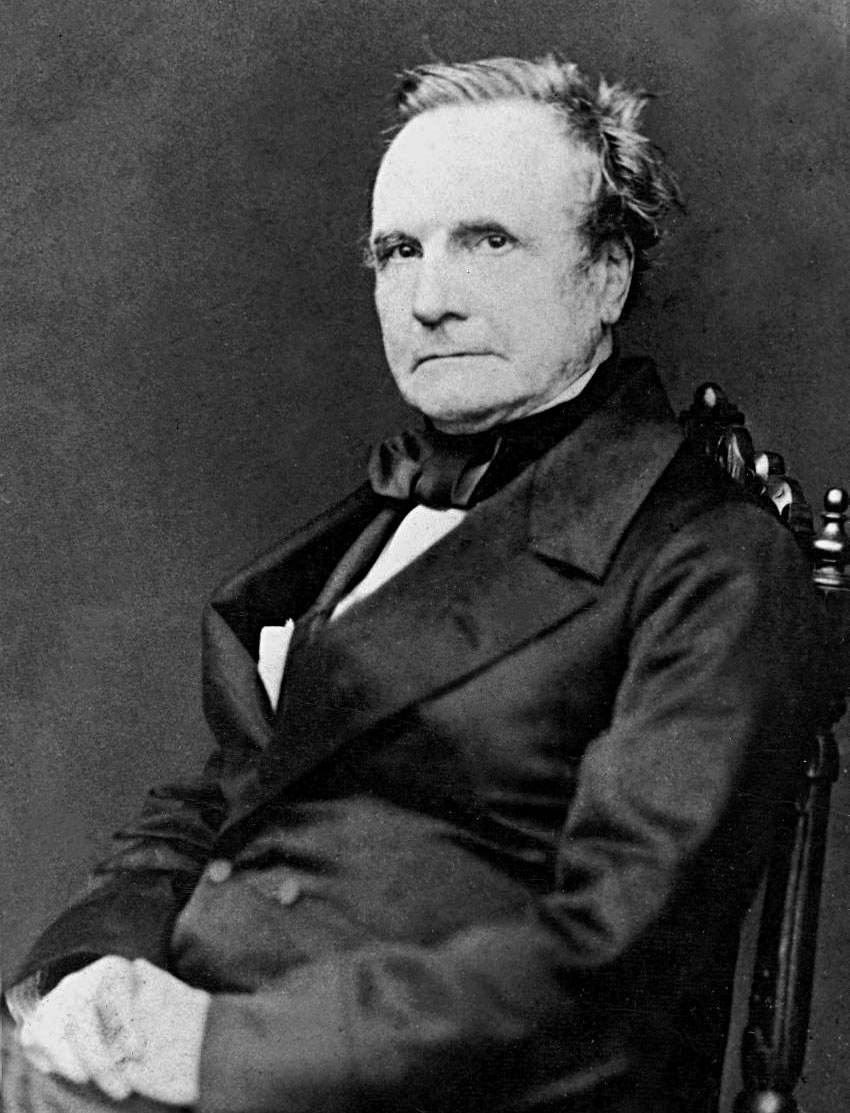
\includegraphics[width=\linewidth]{Charles_Babbage-1860.jpg}
    \end{column}

    \begin{column}{0.6\linewidth}
      \begin{itemize}\cramplist
      \item Considered to be the ``Father of the computer''. Designed
        mechanical machines to compute values of polynomial
        functions. \emph{Not completed in his lifetime}. Built by
        Science Museum, London in 1991 (printer he designed
        constructed in 2000)
        \mypause%
      \item Accomplishment of greatest genius was the invention of the
        ``Analytical Engine''. General purpose computer, with all
        essential ideas now found in modern computer hardware worked
        out in detail.
      \end{itemize}
      See links on lecture website. See also cyberpunk novel ``The
      Difference Engine''. Explores dystopian alternate history in
      which Analytical Engine built.
    \end{column}
  \end{columns}
\end{frame}
%----------------------------------------------------------------

%----------------------------------------------------------------
\begin{frame}{Some History: John von Neumann, (1903-1957)}
  \begin{columns}
    
    \begin{column}{0.4\linewidth}
      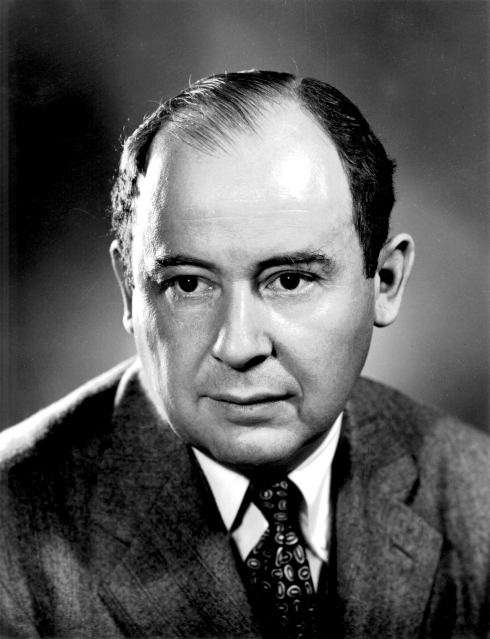
\includegraphics[width=\linewidth]{JohnvonNeumann-LosAlamos.png}
    \end{column}

    \begin{column}{0.6\linewidth}
      \begin{itemize}\cramplist
      \item Polymath of great genius: mathematician, physicist and
        computer scientist. Modern computer architecture (von Neumann
        architecture) named after him.%
        \mypause%
      \item Influential machine designed at Institute of Advanced
        Study from 1945-1951; 40-bit ``word'' with two 20-bit
        instructions; 1024 words of memory.
        \mypause%
      \item Also wrote first and highly influential paper on error
        analysis on Gaussian elimination with Herman Goldstine:
        created field of numerical analysis. See review in SIAM Rev.
        {\bf 53} (4), pp.607-682.
      \end{itemize}
    \end{column}
  \end{columns}
\end{frame}
%----------------------------------------------------------------

%----------------------------------------------------------------
\begin{frame}{Many others, some with Princeton background}
  The history of computing is complex and many people have played key
  role, many with Princeton background (like von Neumann who was at
  IAS)
  \begin{itemize}
  \item Alan Turing. Towering genius in theoretical computer science,
    got his math Ph.D from Princeton University. Invented ``Turing
    machines'', an abstract model for universal computing
    machine. Very influential and part of modern CS curriculum. Worked
    with von Neumann on philosophy of AI and machine computability.%
    \mypause%
  \item Not so well known: Charles Sander Peirce (``Purse''). Realized
    that logical operations could be carried out by {\bf electrical
      circuits, way back in 1886}, decades before such machines were
    built! See letter in which \emph{first logic circuit} is described
    to his former student Allan Marquand of Princeton. (Science
    Library near GIS and book stacks). Rather sad letter, written when
    C.S Peirce was very poor and had to borrow money from Marquand. (Art
    library named after Marquand).
  \end{itemize}
\end{frame}
%----------------------------------------------------------------

%----------------------------------------------------------------
\begin{frame}{A note on computer speeds and prefixes}
  Just a reminder
  \begin{itemize}
  \item Giga = billion ($10^9$)
  \item Tera = trillion ($10^{12}$)
  \item Peta = $10^{15}$
  \item Exa = $10^{18}$ (billion times faster that Gigascale)
  \end{itemize}
  Typical processors are in the GHz range. (My MacBook Pro clocks at
  2.8 GHz and has 4 cores). Typical laptop drives are in terabyte
  range. Largest current machines provide 10s of Petaflops computing
  powers with new exascale machines available in a 2-5 years.
\end{frame}
% ----------------------------------------------------------------

%----------------------------------------------------------------
\begin{frame}{What drives single processor performance?}
  Moore's ``Law'' (more of an industry observation) ``The number of
  transistors incorporated in a chip with approximately double every
  24 months''%
  \footnotesize%
  \begin{columns}
    \begin{column}{0.55\textwidth}
      \begin{figure}
        \incfig{Moores_Law_Transistor_Count_1971-2018.png}
      \end{figure}
    \end{column}
    \begin{column}{0.45\textwidth}
      \begin{itemize}\cramplist
      \item Ultimately, it boils down to the smallest feature sizes
        that can be lithographed. At one point, people thought it
        would bottom out at $28$~nm. However many companies have
        $10$~nm and $7$~nm in mass production, with $5$~nm around the
        corner.
      \item \emph{Eventually, individual processors are not going to
          get much faster}. It is hard to shrink semiconductor feature
        sizes any futher. Fundamental limits from physics (speed of
        light, EM cross-talk, heat generation, ...
      \end{itemize}
    \end{column}
  \end{columns}
\end{frame}
% ----------------------------------------------------------------

%----------------------------------------------------------------
\begin{frame}{At present, processor hardware architecture is in
    significant flux}
  \footnotesize%
  \begin{itemize}
  \item There is a trend away from faster, complex, chips to chips
    with simpler, less fast ``cores'' (many-core machines)
  \item Power consumption is a huge issue with major supercomputer
    installations. If we go along the path we are on now, a small
    power-plant will be required to simply run the cooling systems of
    large machines.
  \item With the rise of handheld devices (smartphones, tablets, ...)
    there is a drive towards low-cost and low-power chips. Significant
    work in ARM chips is going on. (These are Reduced Instruction Set
    Computer (RISC) chips, designed to be cheap and low power)
  \item Use of Graphics Processing Units (GPUs) in HPC is also
    increasing.
  \item It is incredibly hard for software to keep up with
    hardware. Software is written by humans, who need to eat, sleep,
    take vacation, etc. Also, software is \emph{extremely
      complicated}, more so than the hardware it runs on.
  \end{itemize}
  {\color{blue} A major applied mathematics, computational physics and
    software engineering challenge is to design algorithms which take
    advantage of this complicated zoo of emerging hardware.}

\end{frame}
% ----------------------------------------------------------------

%----------------------------------------------------------------
\begin{frame}{Two major types of parallel programming}

  To remain abstract, I will use ``Processing Unit'' (PU) as a
  short-hand. It could mean independent CPUs, threads or cores.
  \begin{itemize}
  \item In \emph{Shared memory} parallel programming, different PUs
    may run different code, but have access to the same
    \emph{memory}. Synchronization of read/writes is a major
    issue.
  \item Shared memory systems usually use ``threads''. These are
    separate code execution paths. A CPU runs a thread for a bit, stops
    it, and then runs another thread. Complex programs can have
    hundreds of threads. %
    \mypause%
  \item In the second type, \emph{distributed memory}, each PU
    executes the same code, but on their own portions of the
    data. Communication is done via \emph{messages}. This is the most
    common pattern in code which solves PDEs (either via grid or PIC
    methods).
  \end{itemize}  
\end{frame}
%----------------------------------------------------------------

%----------------------------------------------------------------
\begin{frame}{How much can parallel algorithms help? Amdahl's Law}

  Amdahl wrote an important paper in 1967 (``Validity of the single
  processor approach to achieving large scale computing
  capabilities''). Basically, he advocates using \emph{serial}
  processing. Paper starts out: {\color{blue} ``For over a decade
    prophets have voiced the contention that the organization of a
    single computer has reached its limits and that truly significant
    advances can be made only by interconnection of a multiplicity of
    computers in such a manner as to permit cooperative
    solution. .... Demonstration is made of the continued validity of
    the single processor approach and of the weaknesses of the
    multiple processor approach in terms of application to real
    problems and their attendant irregularities''}%
  \vskip0.1in%
  This paper has the statement to what is now known as ``Amdahl's
  Law''. It is a very good (and quick) read.%
  \vskip0.1in%
  \mypause%
  Incidentally: Amdahl never actually writes any equations in his
  paper, but states it in words! (Perhaps he didn't know how to
  typeset equations?)

\end{frame}
%----------------------------------------------------------------

%----------------------------------------------------------------
\begin{frame}{Amdahl's Law shows the limitation of parallel
    programming with \emph{constant work loads}}

  Let a process take unit time to run. Then, ideally, with $p$ PUs,
  the run time should be $1/p$. Amdahl points out that in reality,
  only a fraction $f$ can sped up, the remaining $1-f$ is
  ``irreducibly'' serial. Hence, the run-time is
  \begin{align*}
    T_a(p,f) = f/p + (1-f)
  \end{align*}
  Hence, \emph{speedup} will be
  \begin{align*}
    S_a(p,f) = \frac{1}{f/p + (1-f)}
  \end{align*}
  Note that if $f<1$, then
  \begin{align*}
    S_a(\infty,f) = \frac{1}{1-f}
  \end{align*}
  which is independent of number of PUs!

\end{frame}
%----------------------------------------------------------------

%----------------------------------------------------------------
\begin{frame}{Amdahl's Law for various parallelizable fractions}
  \begin{figure}
    \setkeys{Gin}{width=0.6\linewidth,keepaspectratio}
    \incfig{amdahls-law.pdf}
    \caption{Amdahl's Law shows that the speedup of a parallel program
      will quickly saturate if there is any fraction of the work which
      is irreducibly serial.}
  \end{figure}
\end{frame}
%----------------------------------------------------------------

%----------------------------------------------------------------
\begin{frame}{Some comments on Amdahl's Law}
  \begin{itemize}
  \item Amdahl's law is \emph{optimistic} in the sense that it assumes
    that the parallelizable fraction speedup scales linearly. Things
    get worse with (inevitable) overhead say from messaging, etc.%
    \mypause%
  \item Amdahl's law is \emph{pessimistic} in that it assumes that
    \emph{we want faster results for the same problem}. This is not
    true for most problems of interest.
  \end{itemize}
  \mypause%
  In reality, if someone gives us a bigger computer, we want to do a
  \emph{bigger problem}. This is crucial to getting around the
  limitations of Amdahl's Law.%
  \vskip0.1in%
  Assume that if $f$ is the parallelizable fraction of a serial job,
  then with $p$ PUs we will run a $p$ times bigger job. Then, the
  speedup will be
  \begin{align*}
    S_g(p,f) = (1-f) + fp
  \end{align*}
  Note that now, the speedup is linear in $p$! Essentially, the cost
  of the serial part is amortized by going to a bigger problem. This
  is called \emph{Gustafson's Law}.
\end{frame}
%----------------------------------------------------------------

%----------------------------------------------------------------
\begin{frame}{These two speedup laws distinguish \emph{strong} and
    \emph{weak} scaling}

  The \emph{strong scaling} of a problem is the actual speedup one can
  achieve for a problem of fixed size, but increasing PUs. Amdahl's
  law bounds such a scaling. (In general, actual strong-scaling will
  be \emph{worse} than predicted by Amdahl's Law)%
  \mypause%
  \vskip0.1in%
  The \emph{weak scaling} of a problem is the actual speedup one can
  achieve for by problem with size increasing linearly with number of
  PUs. Gustafson's law bounds such a scaling. (In general, actual
  weak-scaling will be \emph{worse} than predicted by Gustafson's
  Law)%
  \mypause%
  \vskip0.1in%
  In general, most real-life problems will scale in a more complicated
  manner. For example, for some problems are I/O and/or communication
  bound. Others are bound by codes which are not parallel at all (for
  example, some old legacy serial code might be needed).

\end{frame}
%----------------------------------------------------------------

%----------------------------------------------------------------
\begin{frame}{The Corollary of Modest Potential}
  This term was coined in an important paper ``Type Architectures,
  Shared Memory, and the Corollary of Modest Potential'' by L. Snyder
  in 1986. (Ann. Rev. Comput. Sci. 1986. 1:289-317).%
  \vskip0.1in%
  Consider a time-dependent 3D problem on a rectangular grid, with $n$
  number of cells in each direction. Then, assuming that the number of
  time-steps to get to a given time is proportional to $n$, the
  computational time will scale as
  \begin{align*}
    T_m(n) \sim n^4
  \end{align*}
  (There are $n^3$ cells, and $n$ steps to take). Hence, even if we
  get linear scaling from Gustafson's law, the scaling of $n$ with
  number of PUs, $p$, will be sub-linear. In this particular case,
  \begin{align*}
    n \sim p^{1/4}
  \end{align*}
  {\color{blue} Hence, to do a problem 100 times bigger, we will need
    $10^8$ more computing resources!}%
\end{frame}
%----------------------------------------------------------------

%----------------------------------------------------------------
\begin{frame}{Can be \emph{worse} than predicted by The
    Corollary of Modest Potential}
  Note that most algorithms are not \emph{parallel in time}! This
  means, that for a 3D problem, we can only use $\sim n^3$ more PUs,
  and need to run for a factor of $n$ longer.
\end{frame}
%----------------------------------------------------------------

%----------------------------------------------------------------
\begin{frame}{What do all of these (seemingly pessimistic) scaling
    laws teach us?}
  This \emph{does not} mean that things are hopeless! In fact, what
  this means is that parallel algorithms must go hand-in-hand with
  better physics models, which do not require such high
  resolutions. For example, 
  \begin{itemize}
  \item Instead of solving Navier-Stokes (NS) equations, one solves
    Reynolds Averaged NS (RANS) equations, or uses Large Eddy
    Simulation (LES) techniques%
    \mypause%
  \item Or, instead of tracking very particle in a large system, one
    performs statistical averaging and uses expensive particle/kinetic
    calculations to provide occasional validation
    \mypause%
  \item Or, instead of doing Vlasov-Maxwell (6D, with plasma frequency
    time-scales), one uses (in appropriate limits) gyrokinetic
    equations (5D, with turbulent fluctuation time-scales), or fluid
    or other appropriate approximations.
  \end{itemize}%
\end{frame}
%----------------------------------------------------------------

%----------------------------------------------------------------
\begin{frame}{Conclusion: Ammar's Corollary of Cynical Progress}

  {\color{blue} It is easy to fill up the biggest computer with FLOPs
    and bytes. It is \emph{much} harder to do useful science.}%
  \vskip0.1in%
  Another way to put it: in a Darwinian process with pressure to use
  bigger-and-bigger machines, one may select for less-than-desired
  traits\footnote{Or, the likely historical 30\% unemployment and
    potential 50\% drop in US GDP due to The Virus will put a final
    halt to Moore's Law and we will be left with our abacuses
    (abacii?) and log tables to compute with. We will know in a few
    months!}.
\end{frame}
% ----------------------------------------------------------------

%----------------------------------------------------------------
\begin{frame}[fragile]{Anatomy of a Very ``Simple'' Problem}

  \myb{Numerical Methods 101: Write a function to multiply two square
    matrices}%
  \vskip0.1in%
  \begin{columns}
    \begin{column}{0.4\linewidth}
\begin{verbatim}
  for (auto i=0; i<N; ++i)
    for (auto j=0; j<N; ++j) {
      C(i,j) = 0.0;
      for (auto k=0; k<N; ++k)
        C(i,j) += A(i,k)*B(k,j);
    }
\end{verbatim}
  \end{column}
  
  \begin{column}{0.5\linewidth}
    Recall that
    \begin{align*}
      C_{ij} = \sum_k A_{ik} B_{kj}
    \end{align*}
    \mypause%
    \vskip0.1in%
    The solution in C++ is very simple: However, how efficient is this
    solution?
  \end{column}
\end{columns}  

\end{frame}
%----------------------------------------------------------------

%----------------------------------------------------------------
\begin{frame}{There is a long history of linear algebra libraries}
  \footnotesize%
  \begin{itemize}
  \item Designing \emph{efficient} linear algebra routines is not
    trivial, even for such ``simple'' matrix-matrix multiply problems.
  \item Most widely used libaries are BLAS (Basic Linear Algebra
    System) on top of which is built LAPACK (Linear Algebra Package).
  \item BLAS provides ``basic'' routines (matrix-vector, matrix-matrix
    multiplication, etc). LAPACK provides linear solvers, eigensystem
    finders, Singular Value Decomposition (SVD), etc.
  \item Created originally by Jack Dongara in 1970s. Continues to be
    developed and optimized. Many platforms (Apple, Intel, ...) supply
    their own highly optimized BLAS/LAPACK libaries. Other
    ``self-tuning'' implementations also exist (see ATLAS).
  \item Modern libraries using very clever C++ techniques are also
    being created and extensively used. The best example I know of is
    the Eigen C++ library (see \url{http://eigen.tuxfamily.org/}).
  \end{itemize}
  \normalsize%
  \myb{Lets compare our hand-written code with Eigen and BLAS. (Look
    at code)}

\end{frame}
% ----------------------------------------------------------------

%----------------------------------------------------------------
\begin{frame}{What do Eigen/BLAS know that we don't?}
  
  {\bf Cache usage and use of SIMD\footnote{Single Instruction
      Multiple Data} instructions}. Modern processors have a hierachy
  of memory locations they can access, with \emph{very} different
  access speeds.%
  \vskip0.1in%
  \footnotesize%
  \begin{columns}
  
    \begin{column}{0.5\linewidth}
      \begin{figure}
        \setkeys{Gin}{width=\linewidth,keepaspectratio}
        \incfig{min-cache.pdf}
        \caption{A very simple cache configuration}
      \end{figure}
    \end{column}
  
    \begin{column}{0.5\linewidth}
      A ``cache'' is an area of memory which is close to the CPU
      core. The memory access to the cache is very fast, compared to
      access to main memory. The difference comes about as main memory
      is Dynamic RAM (DRAM) v/s cache is SRAM. DRAM circuits are tiny
      (hence more of them can be on a single chip) v/s SRAM circuits
      which are very large. However, DRAM essentially relies
      capacitive discharge, which is very slow.
    \end{column}
  \end{columns}

\end{frame}
%----------------------------------------------------------------

%----------------------------------------------------------------
\begin{frame}{Eigen and BLAS preload as much data as possible in the
    fast cache}

  \begin{itemize}
  \item Using clever techniques, these libraries preload as much of
    the matrix data as possible into the cache
  \item Once loaded, the CPU can fetch this data very rapidly to
    do the multiplication and sums.
  \item \myb{On modern CPUS FLOPS are basically free. For example,
      most operations take a single (even fewer) cycle.} It is the
    memory access which is very expensive (~5-20 cycles for cache, and
    100s of cycles for main memory). Hence, to improve performance,
    one must make sure that cache is used in an optimal manner.
  \end{itemize}
\end{frame}
%----------------------------------------------------------------

%----------------------------------------------------------------
\begin{frame}{Why is our matrix-matrix multiply code so slow?}

  {\color{blue} Is it because of the data access pattern in
    matrix-matrix multiply?}

  \begin{figure}
    \setkeys{Gin}{width=0.5\linewidth,keepaspectratio}
    \incfig{mat-access.pdf}
    \caption{In row major order (left) the \emph{rows} are kept
      contigously. To be cache friendly one must increment the row
      index ($i$) faster. In column major order (left) the
      \emph{columns} are kept contigously. To be cache friendly one
      must increment the columns $j$ index faster. \myb{For
        matrix-matrix multiply this is impossible, as one or either
        indexing will incur a cache miss!}}
  \end{figure}

\end{frame}
%----------------------------------------------------------------

%----------------------------------------------------------------
\begin{frame}[fragile]{So how to overcome this seemingly ``impossible''
    situation?}
  \footnotesize%
  \begin{columns}
    
    \begin{column}{0.4\linewidth}
\begin{verbatim}
  // transpose
  Matrix T(N,N);
  for (auto i=0; i<N; ++i)
    for (auto j=0; j<N; ++j)
      T(i,j) = B(j,i);
  
  for (auto i=0; i<N; ++i)
    for (auto j=0; j<N; ++j) {
      C(i,j) = 0.0;
      for (auto k=0; k<N; ++k)
        C(i,j) += A(i,k)*T(j,k);
    }
\end{verbatim}
    \end{column}
    
    \begin{column}{0.6\linewidth}
      The problem is that the matrix-matrix product is an inner
      product of columns of $A$ with the rows of $B$. So, lets
      \myb{copy the \emph{transpose} of $B$ matrix to a temporary
        matrix $T$}. I.e. $T=B^{T}$. Then, the matrix-matrix multiply
      becomes
      \begin{align*}
        C_{ij} = \sum_k A_{ik} T_{jk}
      \end{align*}
      Now, note that if the data is stored in \emph{column} major
      order, both matrices are accessed in a cache friendly manner!%
      \vskip0.1in%
      This is problem and chip dependent: likely does not matter much
      for ``small'' matrix sizes.
    \end{column}
  \end{columns}
\end{frame}
%----------------------------------------------------------------

%----------------------------------------------------------------
\begin{frame}{Modern CPUs very complicated: multiple levels of
    caches, SIMD ...}

  \begin{columns}
  
    \begin{column}{0.6\linewidth}
      \begin{figure}
        \setkeys{Gin}{width=0.8\linewidth,keepaspectratio}
        \incfig{three-level-cache.pdf}
      \end{figure}
    \end{column}
  
    \begin{column}{0.4\linewidth}
      A more realistic processor with three levels of cache. Caches
      further from the CPU core are slower, but larger. On my MacBook
      Pro I have 32KB L1 Cache, 256KB L2 Cache and 6MB L3 Cache. In
      contrast I have 16GB of main memory!
    \end{column}
  \end{columns}  
  
\end{frame}
%----------------------------------------------------------------

\end{document}


\begin{frame}{}
\end{frame}

\begin{columns}
  
  \begin{column}{0.6\linewidth}
  \end{column}
  
  \begin{column}{0.4\linewidth}
    \includegraphics[width=\linewidth]{fig/Kinsey_2011_Pfus_vs_T.pdf}
  \end{column}
\end{columns}

% ----------------------------------------------------------------
